\chapter{Organización de los sistemas nerviosos}\label{ch:b3:nervous-systems}

Una medusa tiene unos pocos miles de neuronas en una red sin centro y
es capaz de nadar, alimentarse y enderezarse. Un pulpo tiene quinientos
millones, dos tercios de ellas en los brazos, cada uno de los cuales
resuelve problemas de los que al cerebro no se le ha informado. El ser
humano tiene ochenta y seis mil millones, unidas por cien billones de
sinapsis, que funcionan con veinte vatios ---una quinta parte de su
energía para el dos por ciento de su masa--- y Santiago Ramón y Cajal,
al dibujarlas célula a célula en la década de 1890 sobre cortes teñidos
con plata, vio que eran células separadas que se tocaban sin fusionarse
y que las señales las recorrían en un solo sentido. El volumen anterior
trató la neurona: su potencial de reposo, su potencial de acción, su
sinapsis. Este capítulo trata aquello en lo que las neuronas están
cableadas: el cable pasivo que limita cuán lejos y cuán rápido se
propaga una señal, los circuitos ---reflejo, oscilador, inhibición
circundante--- con los que se ensambla la conducta, el plan del sistema
nervioso de los vertebrados y de la \omterm{def:b3:nervous-systems:cells}{glía} que lo mantiene en marcha, su
presupuesto energético y las maneras en que distintos animales han
distribuido sus neuronas.

\section{Neuronas y glía}

\begin{definition}[Las células del sistema nervioso]\label{def:b3:nervous-systems:cells}
\index{neurona!tipos}\index{glía}\index{astrocito}\index{oligodendrocito}\index{mielina}\index{microglía}\index{interneurona}
Las neuronas adoptan unas pocas arquitecturas que reaparecen por todo
el encéfalo: las células \emph{piramidales}, las neuronas de proyección
excitadoras de la corteza, con una larga dendrita apical y un axón que
puede recorrer un metro; las células de \emph{Purkinje} del \omterm{def:b3:nervous-systems:plan}{cerebelo},
cuyo árbol dendrítico plano recibe doscientas mil sinapsis; las
neuronas sensitivas, con una prolongación hacia la periferia y otra
hacia la médula; y las \emph{interneuronas}, células de axón corto que
no salen de una región y que en su mayoría son inhibidoras. Cuatro de
cada cinco neuronas corticales liberan glutamato y excitan; una de cada
cinco libera GABA e inhibe. La \emph{glía}, tan numerosa como las
neuronas, hace lo demás. Los \emph{astrocitos} envuelven sinapsis y
vasos sanguíneos: captan el potasio que liberan las neuronas al
descargar y el glutamato que derraman las sinapsis, aportan lactato,
regulan localmente el flujo sanguíneo e inducen y mantienen la \omterm{prop:b3:nervous-systems:barrier-budget}{barrera
hematoencefálica}. Los \emph{oligodendrocitos} del sistema nervioso
central y las \emph{células de Schwann} de la periferia envuelven los
axones en \emph{mielina}, decenas de capas de membrana que aíslan el
axón entre los nódulos donde se sitúan los canales. La
\emph{microglía} está formada por los \omterm{def:b3:innate-immunity:innate}{macrófagos} residentes del
encéfalo, que podan sinapsis durante el desarrollo y retiran los
restos. Las células ependimarias tapizan los ventrículos y fabrican el
\omterm{prop:b3:nervous-systems:barrier-budget}{líquido cefalorraquídeo}.
\end{definition}

\begin{proof}[Evidencia]
La tinción de cromato de plata de Golgi (1873) ennegrecía, por razones
desconocidas, aproximadamente una neurona de cada cien, y la ennegrecía
por completo, dejando invisibles las demás: así podía verse entera una
sola célula en una maraña de millones. Golgi leyó sus propias
preparaciones como un retículo continuo; Cajal, desde 1888, empleando
la misma tinción sobre tejido embrionario, donde las células son más
simples, vio que cada célula terminaba libremente, que dendritas y axón
diferían y que los axones terminaban sobre las dendritas y los cuerpos
de otras células sin unirse a ellas. De la disposición de las células
sensitivas y motoras dedujo el sentido del flujo ---dendrita, cuerpo,
axón---, la \emph{ley de la polarización dinámica}. Sherrington
bautizó el hueco como \emph{sinapsis} en 1897; el microscopio
electrónico lo mostró en 1954.
\end{proof}

\begin{omfigure}
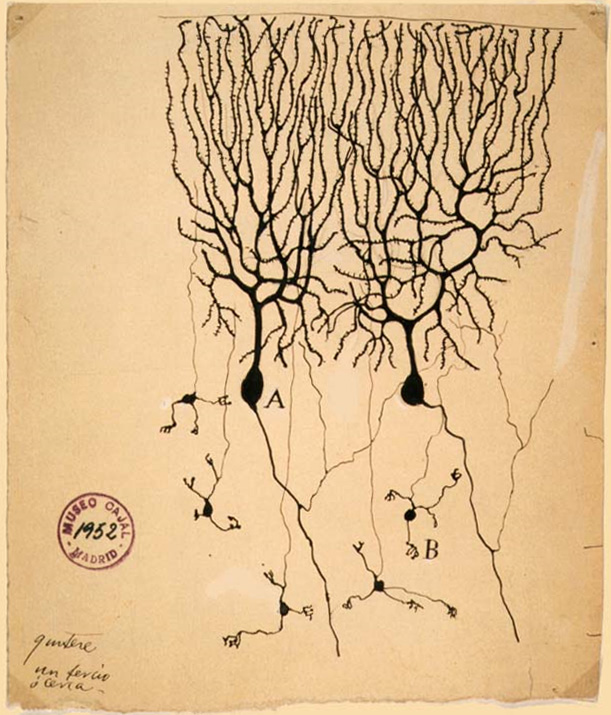
\includegraphics[width=0.30\linewidth]{images/book5/cajal-purkinje.jpg}\hspace{0.04\linewidth}
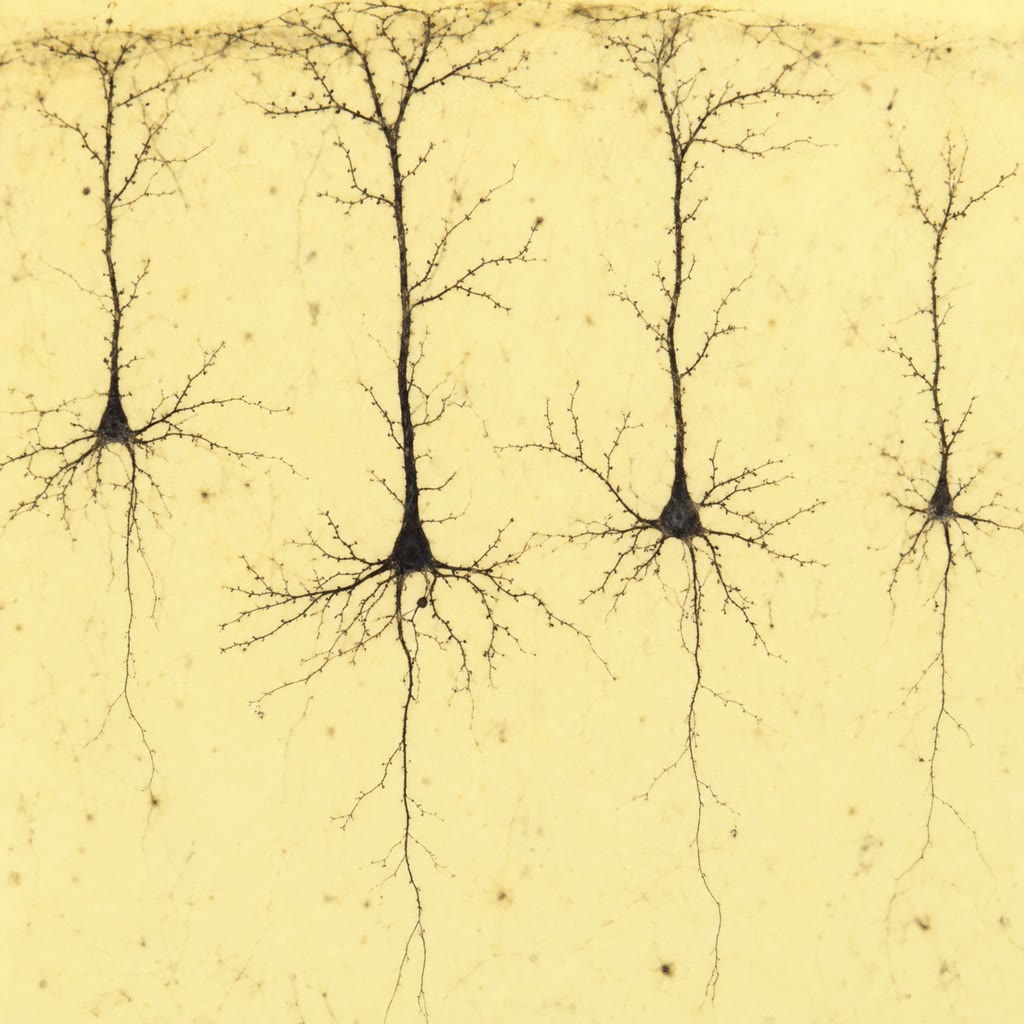
\includegraphics[width=0.30\linewidth]{images/book5/ai/b5-17-cortex-neurons.jpg}\hspace{0.04\linewidth}
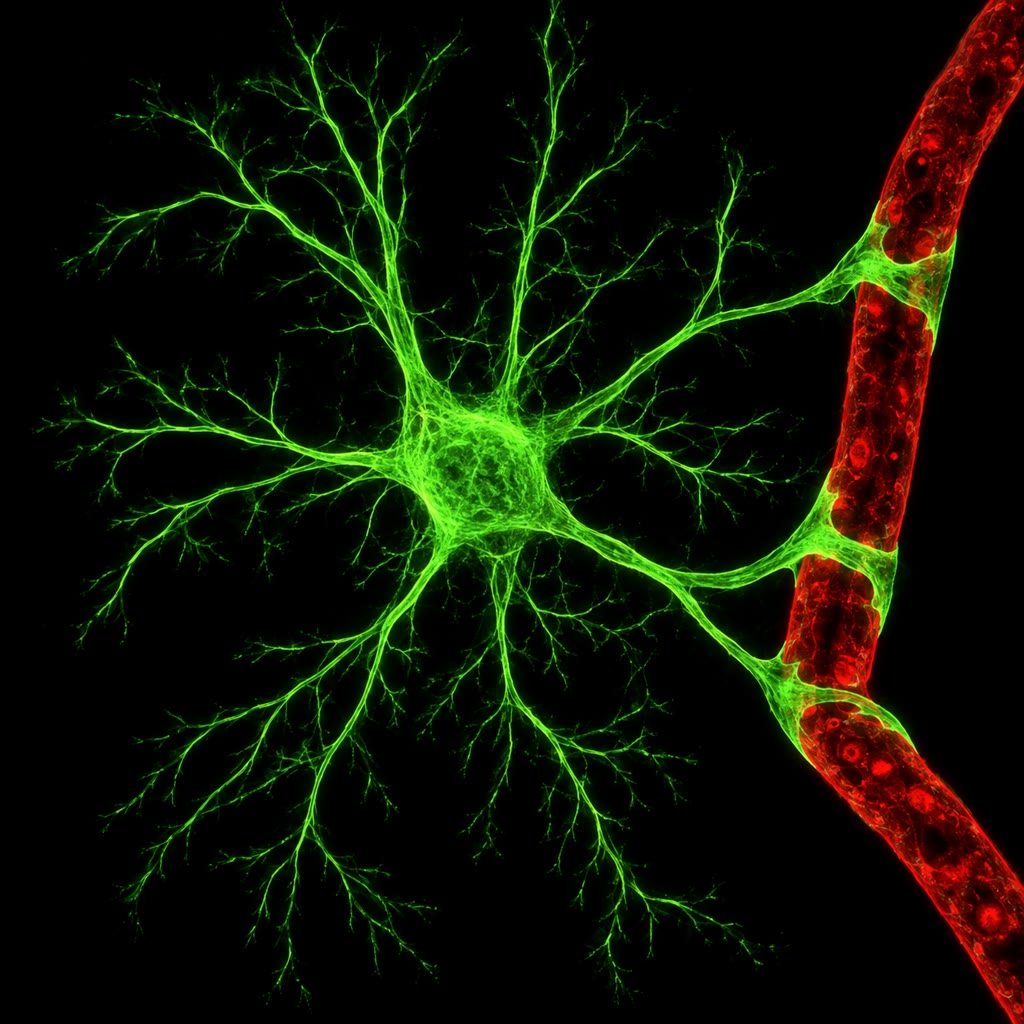
\includegraphics[width=0.30\linewidth]{images/book5/ai/b5-17-astrocyte.jpg}

{\small Izquierda: una célula de Purkinje del \omterm{def:b3:nervous-systems:plan}{cerebelo} dibujada por
Cajal (1899) a partir de un corte teñido con el método de Golgi ---el
árbol dendrítico completo de una sola célula, el argumento a favor de
la neurona como unidad (dominio público). Centro: neuronas piramidales
de la corteza en una tinción de Golgi. Derecha: un \omterm{def:b3:nervous-systems:cells}{astrocito} (verde)
con sus pies terminales sobre un capilar (rojo).}
\end{omfigure}

\section{La neurona como cable}

\begin{theorem}[La ecuación del cable en estado estacionario]\label{thm:b3:nervous-systems:cable}
\index{ecuación del cable}\index{constante de longitud}\index{constante de tiempo!de membrana}\index{velocidad de conducción}
Modélese una dendrita o un axón amielínico como un cilindro de diámetro
$d$ cuyo citoplasma tiene resistividad $R_{i}$ y cuya membrana tiene
resistencia específica $R_{m}$ (resistencia multiplicada por el área) y
capacitancia $C_{m}$ por unidad de área. Por unidad de longitud, la
resistencia axial es $r_{i} = 4R_{i}/\pi d^{2}$ y la resistencia de
membrana, $r_{m} = R_{m}/\pi d$. Un voltaje constante $V_{0}$ aplicado
en $x = 0$ se propaga a lo largo de la fibra como
\[
V(x) = V_{0}\,e^{-x/\lambda}, \qquad
\lambda = \sqrt{\frac{r_{m}}{r_{i}}} = \sqrt{\frac{R_{m}\,d}{4R_{i}}},
\]
donde $\lambda$ es la \emph{\omterm{thm:b3:nervous-systems:cable}{constante de longitud}}: la distancia a lo
largo de la cual una señal pasiva decae a $1/e$, que crece con la raíz
cuadrada del diámetro. La membrana se carga con la \emph{constante de
tiempo} $\tau =
R_{m}C_{m}$, independiente de la geometría. Un potencial de acción, que
se regenera a sí mismo, viaja por un axón amielínico a una velocidad
proporcional a $\lambda/\tau$ y, por tanto, a $\sqrt{d}$; por un axón
mielínico, donde salta de nódulo a nódulo, a una velocidad proporcional
a $d$ ---unos \qty{6}{m/s} por micrómetro de diámetro.
\end{theorem}
\begin{proof}
Sea $I(x)$ la corriente axial. La ley de Ohm a lo largo del núcleo da
$\mathrm{d}V/\mathrm{d}x = -r_{i}I$; la conservación de la carga en
estado estacionario dice que la corriente axial perdida entre $x$ y $x + \mathrm{d}x$
se fuga por la membrana, $\mathrm{d}I/\mathrm{d}x = -V/r_{m}$.
Derivando la primera y sustituyendo la segunda,
$\mathrm{d}^{2}V/\mathrm{d}x^{2} = (r_{i}/r_{m})V = V/\lambda^{2}$, una
ecuación lineal de segundo orden cuya solución acotada cuando $x \to \infty$ es
$V_{0}e^{-x/\lambda}$. Al sustituir $r_{m} = R_{m}/\pi d$ y $r_{i} =
4R_{i}/\pi d^{2}$ resulta $\lambda^{2} = R_{m}d/4R_{i}$. La constante
de tiempo es la de una resistencia y un condensador en paralelo, $r_{m}c_{m} =
(R_{m}/\pi d)(C_{m}\pi d) = R_{m}C_{m}$. En cuanto a las velocidades:
una onda que se regenera debe cargar la membrana una \omterm{thm:b3:nervous-systems:cable}{constante de
longitud} por delante en aproximadamente una constante de tiempo, de
modo que $v \sim \lambda/\tau \propto \sqrt{d}$; entre los nódulos de
un axón mielínico la membrana internodal tiene la resistencia elevada y
la capacitancia reducida por el centenar largo de capas de \omterm{def:b3:nervous-systems:cells}{mielina}, la
longitud del internodo escala con $d$, y el resultado es
$v \propto d$. Se admiten las constantes de proporcionalidad.
\end{proof}

\begin{example}[Números para una dendrita y dos axones]\label{ex:b3:nervous-systems:numbers}
Una dendrita de $d = \qty{2}{\micro m}$ con $R_{m} = \qty{2e4}{\ohm.cm^2}$
y $R_{i} = \qty{100}{\ohm.cm}$: $\lambda = \sqrt{2\times 10^{4}\times
2\times 10^{-4}/400}\ \unit{cm} = \qty{0.1}{cm} = \qty{1}{mm}$ ---un
potencial sináptico en la punta de una dendrita de un milímetro llega
al cuerpo celular con un tercio de su tamaño, y por eso la geometría
del árbol dendrítico forma parte de su cómputo. $\tau = 2\times 10^{4}\times
10^{-6}\,\unit{F/cm^2}\cdot\unit{\ohm.cm^2} = \qty{20}{ms}$, la ventana
dentro de la cual deben llegar las entradas para sumarse. Un axón
gigante de calamar de \qty{500}{\micro m}, amielínico, conduce a unos
\qty{25}{m/s}; para hacer lo mismo un vertebrado emplea un axón
mielínico de \qty{4}{\micro m}, quince mil veces menor en sección
transversal ---la razón de que un nervio de vertebrado pueda llevar
diez mil fibras rápidas en el espacio de un solo axón de calamar. Un
axón motor de \qty{20}{\micro m} conduce a \qty{120}{m/s}; cuando la
esclerosis múltiple le arranca la \omterm{def:b3:nervous-systems:cells}{mielina}, la velocidad cae diez veces
y la conducción puede fallar por completo en los tramos desnudos.
\end{example}

\begin{omfigure}
\begin{tikzpicture}
\begin{axis}[
  width=6.4cm, height=5.2cm,
  axis x line=bottom, axis y line=left,
  xmin=0, xmax=3, ymin=0, ymax=1.05,
  xlabel={distancia (mm)}, ylabel={$V/V_{0}$},
  xlabel style={font=\small, at={(axis description cs:0.5,-0.12)}, anchor=north}, ylabel style={font=\small},
  tick label style={font=\scriptsize}, xtick={0,1,2,3}, ytick={0,0.37,1}, yticklabels={0,$1/e$,1},
  clip=false,
]
\addplot[very thick, omDef, domain=0:3, samples=60] {exp(-x/1.0)};
\addplot[very thick, omThm, domain=0:3, samples=60] {exp(-x/0.5)};
\node[font=\scriptsize, omDef, anchor=south west] at (axis cs:1.2,0.45) {$d = \qty{2}{\micro m}$, $\lambda = \qty{1}{mm}$};
\node[font=\scriptsize, omThm, anchor=north west] at (axis cs:0.8,0.22) {$d = \qty{0.5}{\micro m}$, $\lambda = \qty{0.5}{mm}$};
\end{axis}
\begin{axis}[
  at={(7.6cm,0)}, anchor=south west,
  width=6.4cm, height=5.2cm,
  xmode=log, ymode=log,
  xmin=0.1, xmax=1000, ymin=0.1, ymax=200,
  xlabel={diámetro del axón ($\unit{\micro m}$)}, ylabel={velocidad (m/s)},
  xlabel style={font=\small, at={(axis description cs:0.5,-0.12)}, anchor=north}, ylabel style={font=\small},
  tick label style={font=\scriptsize},
  clip=false,
]
\addplot[very thick, omDef, domain=1:25, samples=2] {6*x};
\addplot[very thick, omThm, domain=0.2:1000, samples=2] {1.1*sqrt(x)};
\fill[omThm] (axis cs:500,25) circle (2pt); \node[font=\scriptsize, anchor=north east] at (axis cs:500,23) {axón gigante de calamar};
\fill[omDef] (axis cs:20,120) circle (2pt); \node[font=\scriptsize, anchor=west] at (axis cs:26,120) {axón motor humano};
\node[font=\scriptsize, omDef, anchor=north west, align=left] at (axis cs:1.2,60) {mielínico: $v \propto d$};
\node[font=\scriptsize, omThm, anchor=north west, align=left] at (axis cs:2,0.7) {amielínico: $v \propto \sqrt{d}$};
\end{axis}
\end{tikzpicture}

{\small Izquierda: decaimiento pasivo de una señal constante a lo largo
de una dendrita, para dos diámetros ---la \omterm{thm:b3:nervous-systems:cable}{constante de longitud} crece
como $\sqrt{d}$. Derecha: \omterm{thm:b3:nervous-systems:cable}{velocidad de conducción} frente al diámetro;
la \omterm{def:b3:nervous-systems:cells}{mielina} permite que una fibra de \qty{4}{\micro m} haga aquello para
lo que un axón amielínico necesita medio milímetro.}
\end{omfigure}

\section{Circuitos}

\begin{definition}[Circuitos elementales]\label{def:b3:nervous-systems:circuits}
\index{arco reflejo}\index{inhibición recíproca}\index{inhibición anterógrada}\index{inhibición por retroalimentación}\index{convergencia}\index{divergencia}
Un \emph{arco reflejo} es el camino más corto de un sensor a un
efector: en el reflejo rotuliano, una aferente del huso muscular entra
en la médula y hace sinapsis directamente sobre las neuronas motoras
del mismo músculo, que lo contraen unos \qty{30}{ms} después del golpe
---una sinapsis, sin cerebro. La misma aferente excita una \omterm{def:b3:nervous-systems:cells}{interneurona}
inhibidora dirigida a las neuronas motoras del músculo antagonista
(\emph{inhibición recíproca}), de modo que la contracción del extensor
no tropieza con la del flexor. La mayoría de los circuitos se
construyen con unos pocos \omterm{def:b3:bioinformatics:motif}{motivos}: la \emph{divergencia}, una neurona
que gobierna muchas, y la \emph{convergencia}, muchas sobre una, que
suma indicios; la \emph{inhibición anterógrada}, en la que una entrada
excita a la vez una diana y una \omterm{def:b3:nervous-systems:cells}{interneurona} que inhibe esa diana un
milisegundo después, lo que afila la respuesta en el tiempo; la
\emph{inhibición por retroalimentación}, en la que la propia salida de
la diana excita una \omterm{def:b3:nervous-systems:cells}{interneurona} que la inhibe, lo que limita la
descarga y, extendido a las vecinas, produce la inhibición lateral que
realza el contraste (\cref{ch:b3:sensory-systems}); y la
\emph{desinhibición}, inhibir a un inhibidor, la manera que tienen los
\omterm{def:b3:nervous-systems:comparative}{ganglios} basales de liberar un movimiento.
\end{definition}

\begin{omfigure}
\begin{tikzpicture}[every node/.style={font=\scriptsize}, >=stealth]
  % spinal cord cross-section (schematic)
  \draw[thick, omDef!60, fill=omDef!8] (5.4,1.5) ellipse (2.0 and 1.5);
  \draw[thick, gray, fill=gray!15] (5.4,1.5) .. controls (4.7,2.4) and (4.0,2.6) .. (4.0,1.9) .. controls (4.0,1.2) and (4.6,0.9) .. (4.8,0.5) .. controls (5.0,0.2) and (5.8,0.2) .. (6.0,0.5) .. controls (6.2,0.9) and (6.8,1.2) .. (6.8,1.9) .. controls (6.8,2.6) and (6.1,2.4) .. (5.4,1.5);
  \node[above] at (5.4,3.05) {médula espinal};
  % muscles
  \draw[thick, omMeth!70!black, fill=omMeth!20] (0.2,0.2) rectangle (1.4,2.0); \node[below, align=center] at (0.8,0.1) {extensor\\(cuádriceps)};
  \draw[thick, omThm!70!black, fill=omThm!15] (0.2,-2.6) rectangle (1.4,-1.4); \node[below, align=center] at (0.8,-2.7) {flexor\\(isquiotibiales)};
  \fill[omProp] (0.8,1.3) ellipse (0.12 and 0.3); \node[left, font=\tiny] at (0.65,1.3) {huso};
  % Ia afferent to cord (dorsal)
  \draw[very thick, omProp] (0.9,1.3) .. controls (2.0,2.6) and (3.6,2.9) .. (4.8,2.2); \fill[omProp] (4.8,2.2) circle (0.09);
  \node[above, omProp] at (2.6,2.85) {aferente Ia: estiramiento};
  % motor neuron to extensor
  \fill[omMeth!70!black] (5.0,0.9) circle (0.16);
  \draw[->, very thick, omMeth!70!black] (4.9,0.85) .. controls (3.4,0.3) and (2.0,0.4) .. (1.4,1.0);
  \draw[->, thick, omProp] (4.8,2.2) -- (5.0,1.1);
  % inhibitory interneuron to flexor motor neuron
  \fill[omThm] (6.1,1.7) circle (0.13);
  \draw[->, thick, omProp] (4.9,2.25) -- (6.0,1.8);
  \fill[omThm!70!black] (6.0,0.6) circle (0.16);
  \draw[-|, thick, omThm] (6.1,1.55) -- (6.0,0.8);
  \draw[->, very thick, omThm!70!black, dashed] (5.9,0.5) .. controls (4.8,-0.8) and (3.0,-1.6) .. (1.4,-2.0);
  % right-hand labels with leaders
  \node[right, omThm, font=\tiny] at (7.6,1.9) {interneurona inhibidora Ia}; \draw[gray, thin] (7.55,1.9) -- (6.25,1.7);
  \node[right, omMeth!70!black, font=\tiny, align=left] at (7.6,1.1) {neurona motora del extensor: excitada}; \draw[gray, thin] (7.55,1.1) -- (5.15,0.9);
  \node[right, omThm!70!black, font=\tiny, align=left] at (7.6,0.3) {neurona motora del flexor: inhibida}; \draw[gray, thin] (7.55,0.3) -- (6.15,0.6);
  \node[below] at (4.6,-0.15) {reflejo monosináptico: $\sim$\qty{30}{ms}};
  \node[below, align=center] at (4.2,-2.0) {inhibición recíproca:\\el antagonista se relaja};
\end{tikzpicture}

{\small El reflejo de estiramiento. Un golpe estira los husos del
extensor; la aferente Ia excita directamente las neuronas motoras del
extensor (una sinapsis) y, a través de una \omterm{def:b3:nervous-systems:cells}{interneurona} inhibidora,
silencia las del flexor.}
\end{omfigure}

\begin{proposition}[Generadores centrales de patrones]\label{prop:b3:nervous-systems:cpg}
\index{generador central de patrones}\index{oscilador de semicentros}
Los movimientos rítmicos ---respirar, caminar, nadar, masticar--- los
producen circuitos del \omterm{def:b3:nervous-systems:plan}{tronco encefálico} y de la \omterm{def:b3:nervous-systems:plan}{médula espinal} que
oscilan por sí solos, los \emph{\omterm{prop:b3:nervous-systems:cpg}{generadores centrales de patrones}}, que
la retroalimentación sensitiva ajusta pero no crea: la \omterm{def:b3:nervous-systems:plan}{médula espinal}
de un gato, separada del encéfalo y privada de sus nervios sensitivos,
sigue produciendo el patrón alterno de la marcha. El diseño más simple
es el \emph{semicentro} de Brown (1911): dos grupos de neuronas que se
inhiben mutuamente. El que descarga silencia a su compañero; pero un
grupo que descarga se fatiga ---sus canales se inactivan, su inhibición
del compañero se debilita--- y el compañero, liberado, descarga y a su
vez silencia al primero: alternancia, con un período fijado por la
constante de tiempo de la fatiga y no por reloj alguno. El ritmo
respiratorio surge en un grupo de unos pocos miles de neuronas del
bulbo raquídeo (el complejo pre-Bötzinger), que descarga en ráfagas
desde el nacimiento hasta la muerte; la natación de la lamprea es una
cadena de semicentros a lo largo de su médula, cada uno retrasado
respecto del anterior para que una onda viaje hacia la cola.
\end{proposition}

\begin{omfigure}
\begin{tikzpicture}[every node/.style={font=\scriptsize}, >=stealth]
  % half-centre
  \begin{scope}
    \draw[thick, fill=omDef!25] (0,0) circle (0.5); \node at (0,0) {I};
    \draw[thick, fill=omThm!25] (3,0) circle (0.5); \node at (3,0) {D};
    \draw[-|, very thick] (0.5,0.2) -- (2.5,0.2); \draw[-|, very thick] (2.5,-0.2) -- (0.5,-0.2);
    \node[above] at (1.5,0.3) {inhibición mutua};
    \draw[->, thick, omDef] (0,-0.5) -- (0,-1.3) node[below] {músculos izquierdos};
    \draw[->, thick, omThm] (3,-0.5) -- (3,-1.3) node[below] {músculos derechos};
    \draw[->, thick, gray] (-1.2,0.6) -- (-0.45,0.25) node[pos=0, above, align=center] {impulso tónico\\del tronco encefálico};
    \draw[->, thick, gray] (4.5,0.6) -- (3.45,0.25);
  \end{scope}
  % traces
  \begin{scope}[xshift=6.0cm, yshift=0.9cm]
    \node[left, omDef] at (0,0) {I};
    \foreach \x in {0,2,4} { \foreach \s in {0.1,0.2,...,0.9} \draw[omDef] (\x+\s,-0.15) -- (\x+\s,0.15); }
    \node[left, omThm] at (0,-1.0) {D};
    \foreach \x in {1,3,5} { \foreach \s in {0.1,0.2,...,0.9} \draw[omThm] (\x+\s,-1.15) -- (\x+\s,-0.85); }
    \draw[->] (0,-1.6) -- (6.2,-1.6) node[right] {tiempo};
    \draw[<->] (0,-2.0) -- (2,-2.0) node[midway, below] {período: lo fija la fatiga};
  \end{scope}
\end{tikzpicture}

{\small Un \omterm{prop:b3:nervous-systems:cpg}{oscilador de semicentros}. Dos grupos que se inhiben
mutuamente bajo un impulso constante se alternan: el lado activo se
fatiga, su inhibición se debilita, el otro lado escapa y toma el
relevo. Ninguna neurona es rítmica por sí misma.}
\end{omfigure}

\begin{method}[Trazar un circuito]\label{met:b3:nervous-systems:tracing}
\index{trazado de circuitos}\index{optogenética}
Para establecer que la neurona A gobierna la neurona B y que la vía
importa para una conducta: (1) anatomía ---inyéctese un trazador que
viaje por los axones (un colorante, un \omterm{def:b3:virology:virus}{virus} de la rabia modificado que
cruza una sola sinapsis hacia atrás) y localícense las células
conectadas; (2) fisiología ---regístrese B mientras se estimula A, y
mídanse la latencia (una conexión monosináptica da un retraso fijo de
aproximadamente un milisegundo) y el signo (excitación o inhibición);
(3) necesidad ---silénciese A, por lesión, por enfriamiento o
expresando en ella una bomba de cloruro accionada por luz e
iluminándola (\emph{optogenética}), y véase si la conducta fracasa; (4)
suficiencia ---actívese A sola, con un canal catiónico accionado por
luz, y véase si la conducta aparece; (5) en un animal intacto,
obsérvese la actividad de toda la población con un indicador de calcio
mientras se ejecuta la conducta. Un circuito queda establecido cuando
las cinco cosas concuerdan; la mayoría de los circuitos publicados
tienen dos o tres.
\end{method}

\section{El plan del sistema nervioso de los vertebrados}

\begin{definition}[Divisiones central y periférica]\label{def:b3:nervous-systems:plan}
\index{médula espinal}\index{tronco encefálico}\index{cerebelo}\index{tálamo}\index{hipotálamo}\index{corteza cerebral}\index{sistema nervioso autónomo}\index{sistema nervioso entérico}
El \emph{sistema nervioso central} es el encéfalo y la médula espinal;
el \emph{periférico} es todo lo demás. La \emph{médula espinal} recibe
axones sensitivos por sus raíces dorsales y envía axones motores por
sus raíces ventrales; su sustancia gris es una mariposa de cuerpos
celulares y su sustancia blanca, los tractos mielínicos que suben y
bajan. El \emph{tronco encefálico} ---bulbo, protuberancia,
mesencéfalo--- alberga los núcleos de los nervios craneales y los
centros que mantienen la respiración, la frecuencia cardíaca y la
presión arterial sin intervención del pensamiento; una muerte del
tronco encefálico es la muerte. El \emph{cerebelo}, con más neuronas
que todo el resto del encéfalo, ajusta la sincronía y la coordinación
del movimiento y aprende del error. El \emph{tálamo} transmite a la
corteza todos los sentidos salvo el olfato, y de vuelta las respuestas
de la corteza; el \emph{hipotálamo}, situado debajo, gobierna la
homeostasis ---temperatura, hambre, sed, el reloj, los ejes endocrinos
del \cref{ch:b3:endocrinology}. Los \emph{\omterm{def:b3:nervous-systems:comparative}{ganglios} basales} seleccionan
entre las acciones posibles; el \emph{hipocampo} fabrica los recuerdos
(\cref{ch:b3:learning-memory}); y la \emph{corteza cerebral}, una
lámina de seis capas de células, de dos a cuatro milímetros de grosor y
un cuarto de metro cuadrado de superficie, plegada para caber, hace lo
demás, en áreas cartografiadas para cada sentido y cada movimiento y en
áreas de asociación entre ellas. La división \emph{autónoma} del
sistema periférico gobierna los órganos: la cadena \emph{simpática},
que libera noradrenalina, moviliza (corazón acelerado, intestino
frenado, pupilas abiertas); los nervios \emph{parasimpáticos}, que
liberan acetilcolina, conservan y digieren; y el sistema nervioso
\emph{entérico}, quinientos millones de neuronas en la pared
intestinal, gobierna la digestión por su cuenta.
\end{definition}

\begin{omfigure}
\begin{tikzpicture}[every node/.style={font=\scriptsize}, >=stealth]
  % sagittal brain schematic
  \draw[thick, omDef!70, fill=omDef!15] (0,2.0) .. controls (0,4.6) and (3.5,5.4) .. (6.0,4.4) .. controls (7.6,3.7) and (7.4,2.2) .. (6.2,1.9) .. controls (5.4,1.7) and (5.2,1.3) .. (4.4,1.6) .. controls (3.0,1.3) and (1.2,1.4) .. (0,2.0);
  \node[align=center] at (3.0,3.9) {corteza cerebral: seis capas,\\áreas sensitivas, motoras y de asociación};
  % basal ganglia / hippocampus (deep)
  \draw[thick, omProp!70, fill=omProp!25] (3.2,2.6) ellipse (0.9 and 0.45); \node[font=\tiny] at (3.2,2.6) {ganglios basales};
  \draw[thick, omProp!70, fill=omProp!25] (5.2,2.45) ellipse (0.88 and 0.3); \node[font=\tiny] at (5.2,2.45) {hipocampo};
  % thalamus, hypothalamus
  \draw[thick, omMeth!70!black, fill=omMeth!25] (4.0,1.95) ellipse (0.7 and 0.3); \node[font=\tiny] at (4.0,1.95) {tálamo};
  \draw[thick, omMeth!70!black, fill=omMeth!40] (4.0,1.42) ellipse (0.78 and 0.22); \node[font=\tiny] at (4.0,1.42) {hipotálamo};
  % cerebellum
  \draw[thick, omThm!70, fill=omThm!20] (6.6,1.2) ellipse (0.9 and 0.6); \node[font=\tiny] at (6.6,1.2) {cerebelo};
  % brainstem
  \draw[thick, gray!70, fill=gray!20] (4.7,1.2) -- (5.5,1.2) -- (5.9,-0.3) -- (5.1,-0.3) -- cycle; \node[font=\tiny, rotate=-75] at (5.3,0.45) {tronco encefálico};
  % spinal cord
  \draw[thick, gray!70, fill=gray!20] (5.2,-0.3) rectangle (5.8,-1.6); \node[right, font=\tiny] at (5.85,-1.0) {médula espinal};
  % labels with leaders on the right
  \node[right, align=left] at (7.8,3.4) {tálamo: relevo de todos los\\sentidos salvo el olfato; hipotálamo:\\homeostasis, reloj, ejes endocrinos};
  \draw[gray] (7.75,3.3) -- (4.7,1.95);
  \node[right, align=left] at (7.8,1.9) {cerebelo: sincronía y\\coordinación, aprendizaje del error};
  \draw[gray] (7.75,1.8) -- (7.5,1.4);
  \node[right, align=left] at (7.8,0.4) {tronco encefálico: respiración,\\corazón, nervios craneales (bulbo,\\protuberancia, mesencéfalo)};
  \draw[gray] (7.75,0.4) -- (5.9,0.4);
  \node[right, align=left] at (7.8,-1.0) {médula espinal: reflejos, generadores\\de patrones, tractos ascendentes y descendentes};
\end{tikzpicture}

{\small El encéfalo de los vertebrados en corte sagital, de forma
esquemática: la corteza sobre los núcleos profundos, el \omterm{def:b3:nervous-systems:plan}{tálamo} y el
\omterm{def:b3:nervous-systems:plan}{hipotálamo} en el centro, el \omterm{def:b3:nervous-systems:plan}{cerebelo} detrás, el \omterm{def:b3:nervous-systems:plan}{tronco encefálico} que
continúa en la médula.}
\end{omfigure}

\begin{proposition}[La barrera hematoencefálica y el presupuesto del encéfalo]\label{prop:b3:nervous-systems:barrier-budget}
\index{barrera hematoencefálica}\index{líquido cefalorraquídeo}\index{presupuesto energético del encéfalo}
Los capilares del encéfalo están sellados por uniones estrechas entre
sus células endoteliales, envueltos en pies terminales de \omterm{def:b3:nervous-systems:cells}{astrocito} y
dotados de transportadores que admiten glucosa y aminoácidos y expulsan
casi todo lo demás: la \emph{\omterm{prop:b3:nervous-systems:barrier-budget}{barrera hematoencefálica}}, que mantiene
constante la composición iónica del líquido extracelular del encéfalo
en beneficio del comportamiento eléctrico de las neuronas y que excluye
la mayoría de los fármacos (\qty{98}{\%} de las moléculas pequeñas,
todos los \omterm{def:b3:adaptive-immunity:antibody}{anticuerpos}) ---el problema central de la neurofarmacología.
El encéfalo flota en \qty{150}{mL} de \emph{\omterm{prop:b3:nervous-systems:barrier-budget}{líquido cefalorraquídeo}},
fabricado a medio mililitro por minuto y renovado cuatro veces al día,
que lo amortigua y se lleva los desechos, sobre todo durante el sueño.
El coste del encéfalo: unos \qty{20}{W} en un adulto, el \qty{20}{\%}
del metabolismo de reposo, casi todo en forma de glucosa quemada hasta
ATP, y la mayor parte de ese ATP la gasta la bomba de sodio al
restablecer los gradientes que agotan los potenciales de acción y las
corrientes sinápticas. A \qty{50}{kJ} por mol de ATP, \qty{20}{W} son $4\times 10^{-4}$ mol
de ATP por segundo, $2.4\times 10^{20}$ moléculas; repartidas entre
$8.6\times 10^{10}$ neuronas, unos $3\times 10^{9}$ ATP por neurona y
segundo. Un potencial de acción cortical con sus consecuencias
sinápticas cuesta del orden de $10^{9}$ ATP, de modo que el presupuesto
admite una frecuencia media de descarga de unas pocas espigas por
segundo y neurona ---y las neuronas corticales descargan más o menos a
ese ritmo. El encéfalo está construido con un límite energético
estricto, y por eso sus señales son escasas, sus axones finos y su
información está codificada por pocas espigas en muchas células.
\end{proposition}
\admitted

\section{Los sistemas nerviosos a lo largo del reino animal}

\begin{definition}[Redes nerviosas, ganglios y encéfalos]\label{def:b3:nervous-systems:comparative}
\index{red nerviosa}\index{ganglio}\index{cefalización}\index{encefalización}
Los cnidarios (medusas, hidras) tienen una \emph{red nerviosa}:
neuronas distribuidas por la pared del cuerpo, conectadas en todas
direcciones, con condensaciones anulares alrededor del borde de la
umbrela que coordinan la natación ---sin centro, y con conducción en
ambos sentidos a lo largo de cada célula. Los animales bilaterales
concentran las neuronas en \emph{ganglios} ---agrupaciones con un
neurópilo común--- dispuestos a lo largo de un cordón ventral en
artrópodos y anélidos, con un ganglio cefálico agrandado allí donde
están los órganos de los sentidos: la \emph{cefalización}. Los moluscos
van desde los ganglios simples de una almeja hasta el pulpo, cuyos
quinientos millones de neuronas son las más numerosas de cualquier
invertebrado y dos tercios de las cuales están en los brazos, con el
cordón de cada brazo gobernando su propio alcanzar y agarrar. Los
vertebrados construyen un tubo dorsal hueco, expandido por delante en
el encéfalo de la sección anterior, protegido por hueso y por una
barrera, y mielinizado. Las mismas moléculas de señalización, los
mismos canales y transmisores y muchos de los mismos genes del
desarrollo (el código Hox del rombencéfalo, los factores que modelan el
ojo) rigen todos ellos: las piezas son antiguas y compartidas; las
disposiciones, diversas.
\end{definition}

\begin{example}[Contar neuronas]\label{ex:b3:nervous-systems:counts}
Un nematodo tiene $302$ neuronas, todas ellas con nombre y todas sus
sinapsis cartografiadas; una mosca del vinagre, $1.4\times 10^{5}$; una
abeja, $10^{6}$; un ratón, $7\times 10^{7}$; un pulpo,
$5\times 10^{8}$; un ser humano, $8.6\times
10^{10}$; un elefante, $2.6\times 10^{11}$, la mayoría de ellas en su
\omterm{def:b3:nervous-systems:plan}{cerebelo}. La masa del encéfalo escala con la masa corporal en los
mamíferos aproximadamente como
$M_{\text{cerebro}} \propto M_{\text{cuerpo}}^{0.75}$, de modo que el
encéfalo de un ratón es una fracción mayor de su cuerpo que el de un
elefante; de las especies situadas por encima de la recta para su talla
---delfines, primates, el ser humano por un factor de siete--- se dice
que están encefalizadas. Lo que mejor acompaña a la cognición no es la
masa del encéfalo, sino el número de neuronas de la \omterm{def:b3:nervous-systems:plan}{corteza cerebral}:
unos $1.6\times 10^{10}$ en un ser humano, $5.6\times 10^{9}$ en el
elefante, cuyo encéfalo es tres veces mayor, y $2\times 10^{9}$ en un
chimpancé. El encéfalo humano no es especial ni en sus células ni en su
plan; tiene más neuronas corticales que ningún otro, empaquetadas más
densamente, y parece ser el número, y no el peso, lo que cuenta.
\end{example}

\begin{omfigure}
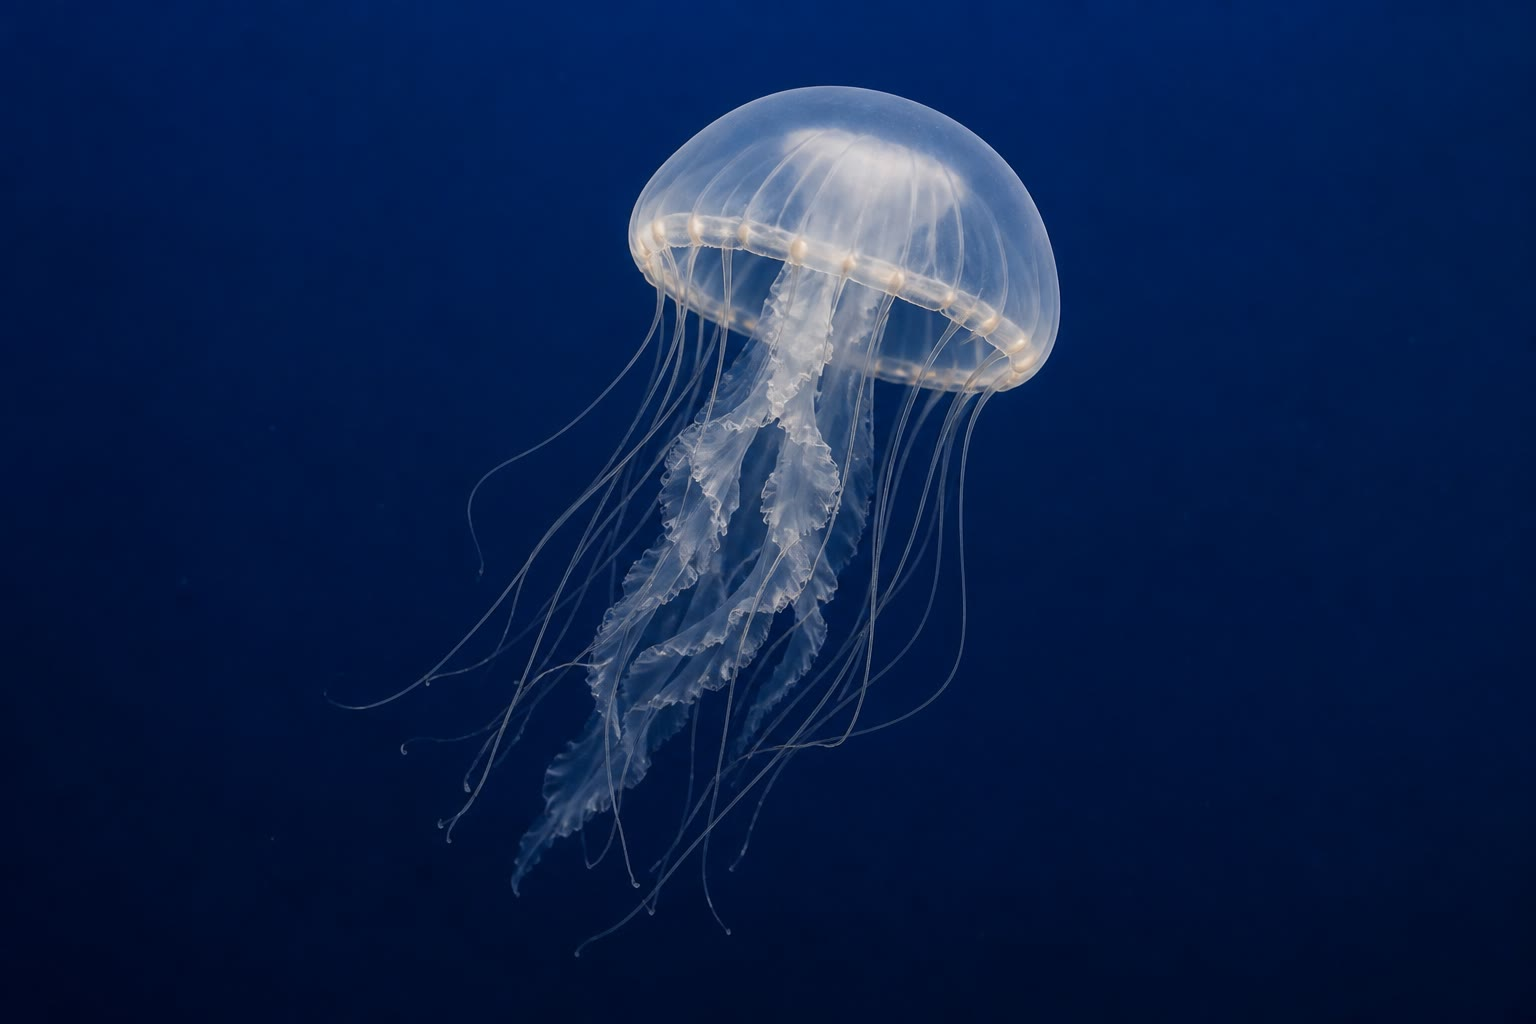
\includegraphics[width=0.46\linewidth]{images/book5/ai/b5-17-jellyfish.jpg}\hspace{0.04\linewidth}
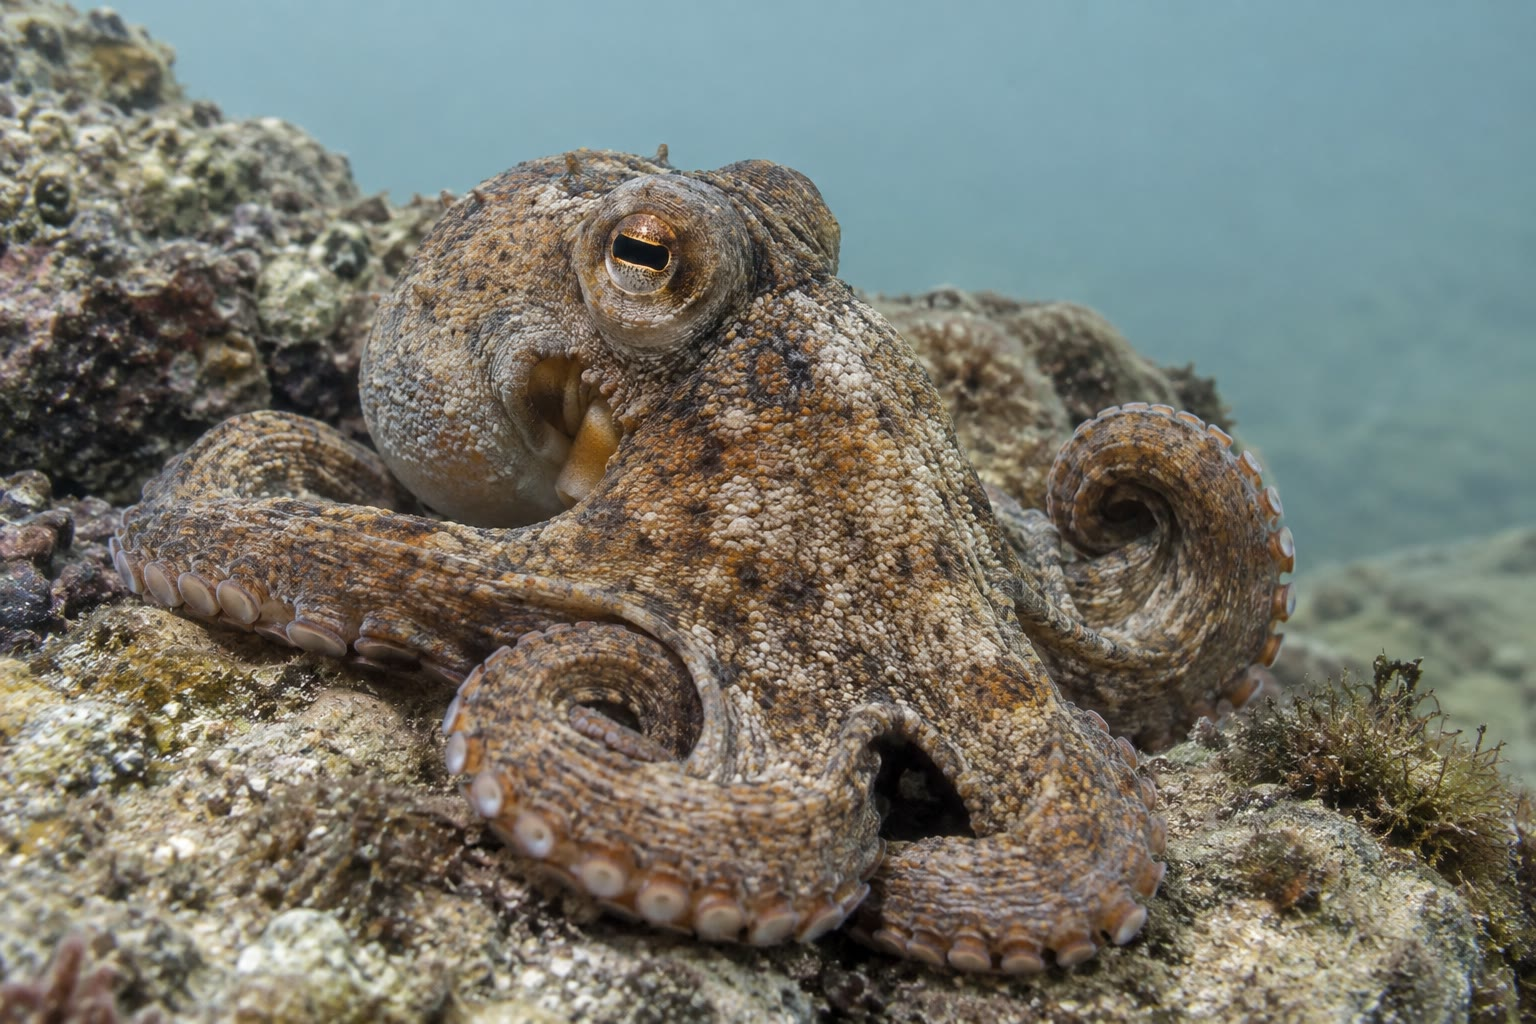
\includegraphics[width=0.46\linewidth]{images/book5/ai/b5-17-octopus.jpg}

{\small Dos maneras de organizar neuronas. Izquierda: una medusa, cuya
\omterm{def:b3:nervous-systems:comparative}{red nerviosa} y cuyos anillos marginales coordinan la natación sin
encéfalo. Derecha: un pulpo, con quinientos millones de neuronas, la
mayoría en los brazos, y el mayor encéfalo de cualquier invertebrado.}
\end{omfigure}

\begin{remark}[Para qué sirve un sistema nervioso]\label{rem:b3:nervous-systems:for}
Las plantas, los hongos y las esponjas no tienen ninguno; un animal que
se mueve necesita uno, y la elaboración de los sistemas nerviosos sigue
las exigencias del movimiento, de la detección a distancia y de la
predicción de lo que va a ocurrir. La \omterm{thm:b3:nervous-systems:cable}{ecuación del cable} fija la física
---cuán lejos y cuán rápido viaja una señal para un diámetro y un
aislamiento dados---; el presupuesto energético fija la economía; y
dentro de esos límites las mismas neuronas, dispuestas en redes,
\omterm{def:b3:nervous-systems:comparative}{ganglios} o una corteza, producen la pulsación de una medusa, el
camuflaje de un pulpo o esta frase. Los dos capítulos siguientes toman
el extremo de entrada y el almacenamiento: cómo los sentidos convierten
el mundo en espigas y cómo cambian las sinapsis para que el mundo, una
vez encontrado, quede recordado.
\end{remark}

\section{Ejercicios}

\begin{exercise}[$\star$]\label{exo:b3:nervous-systems:1}
Nómbrense los cuatro tipos de \omterm{def:b3:nervous-systems:cells}{glía} y una función de cada uno, y dígase
cuáles dos fabrican \omterm{def:b3:nervous-systems:cells}{mielina} y dónde.
\end{exercise}

\begin{exercise}[$\star$]\label{exo:b3:nervous-systems:2}
¿Qué hizo posible la tinción de Golgi, qué concluyó Cajal a partir de
ella y qué concluyó Golgi? ¿Cuál acertó y cómo se zanjó la cuestión?
\end{exercise}

\begin{exercise}[$\star$]\label{exo:b3:nervous-systems:3}
Descríbase el \omterm{def:b3:nervous-systems:circuits}{arco reflejo} rotuliano y explíquese por qué tarda solo
\qty{30}{ms} mientras que una patada voluntaria tarda diez veces más.
\end{exercise}

\begin{exercise}[$\star$]\label{exo:b3:nervous-systems:4}
Enumérense los efectos simpáticos y parasimpáticos sobre el corazón, la
pupila, el intestino y las vías respiratorias, y el transmisor que
emplea cada división en la diana.
\end{exercise}

\begin{exercise}[$\star\star$]\label{exo:b3:nervous-systems:5}
Calcúlese la \omterm{thm:b3:nervous-systems:cable}{constante de longitud} de un axón de \qty{1}{\micro m} con $R_{m}
= \qty{1e4}{\ohm.cm^2}$ y $R_{i} = \qty{100}{\ohm.cm}$, y la fracción
de señal que queda tras \qty{2}{mm}. ¿Qué diámetro duplicaría
$\lambda$?
\end{exercise}

\begin{exercise}[$\star\star$]\label{exo:b3:nervous-systems:6}
Un axón sensitivo de \qty{12}{\micro m} recorre \qty{1.2}{m} desde el
dedo del pie hasta la médula, y un axón motor de \qty{15}{\micro m}
vuelve. Con \qty{6}{m/s} por micrómetro y \qty{0.5}{ms} por sinapsis,
estímese la latencia mínima de un reflejo espinal de retirada con una
\omterm{def:b3:nervous-systems:cells}{interneurona}. ¿Cuánto tardaría con axones amielínicos del mismo
diámetro a $v = 1.1\sqrt{d}$?
\end{exercise}

\begin{exercise}[$\star\star$]\label{exo:b3:nervous-systems:7}
Con el presupuesto del encéfalo de
\cref{prop:b3:nervous-systems:barrier-budget}, estímese cuántos ATP
puede gastar una neurona por segundo y, si una espiga con sus sinapsis
cuesta $2\times 10^{9}$ ATP, la frecuencia media de descarga que
permite el presupuesto. ¿Qué predice esto sobre el código?
\end{exercise}

\begin{exercise}[$\star\star$]\label{exo:b3:nervous-systems:8}
Explíquese por qué un \omterm{prop:b3:nervous-systems:cpg}{oscilador de semicentros} necesita fatiga (u otro
proceso lento) para oscilar, y qué ocurriría con dos neuronas que se
inhiben mutuamente y nunca se cansan.
\end{exercise}

\begin{exercise}[$\star\star$]\label{exo:b3:nervous-systems:9}
La \omterm{prop:b3:nervous-systems:barrier-budget}{barrera hematoencefálica} excluye la dopamina, producto de la L-dopa,
pero admite la L-dopa. Explíquese cómo se aprovecha esto en la
enfermedad de Parkinson y por qué es difícil administrar \omterm{def:b3:adaptive-immunity:antibody}{anticuerpos}
contra proteínas encefálicas.
\end{exercise}

\begin{exercise}[$\star\star\star$]\label{exo:b3:nervous-systems:10}
Dedúzcase la forma dependiente del tiempo de la \omterm{thm:b3:nervous-systems:cable}{ecuación del cable}, $\lambda^{2}\,\partial^{2}
V/\partial x^{2} = \tau\,\partial V/\partial t + V$, sumando la
corriente capacitiva a la corriente de membrana, y muéstrese que de
ella se sigue la solución estacionaria del teorema. Basta con enunciar
la forma; no se pide resolverla. ¿Por qué el cociente $\lambda/\tau$ es
una velocidad?
\end{exercise}

\begin{exercise}[$\star\star\star$]\label{exo:b3:nervous-systems:11}
Un axón gigante de calamar de \qty{500}{\micro m} conduce a
\qty{25}{m/s}. Con $v \propto \sqrt{d}$, ¿qué diámetro de axón
amielínico haría falta para \qty{100}{m/s}? Calcúlese la sección
transversal y compárese con el axón mielínico de \qty{20}{\micro m} que
lo consigue. ¿Qué implica esto sobre el número de fibras rápidas que
puede llevar un nervio y sobre la evolución de la \omterm{def:b3:nervous-systems:cells}{mielina}?
\end{exercise}

\begin{exercise}[$\star\star\star$]\label{exo:b3:nervous-systems:12}
La masa del encéfalo escala como $M_{\text{cuerpo}}^{0.75}$ en los
mamíferos. Un ratón de \qty{30}{g} tiene un encéfalo de \qty{0.4}{g}.
Predígase la masa encefálica de un mamífero de \qty{70}{kg} situado
sobre la recta, compárese con los \qty{1350}{g} humanos y discútase por
qué el número de neuronas corticales, y no la masa del encéfalo, es el
mejor correlato de la capacidad cognitiva.
\end{exercise}

\section{Problema: el cableado de un cuerpo}

\begin{problem}[{Problema de fin de semana --- el cableado de un cuerpo
valorado en constantes de longitud, milisegundos y vatios: los números
del cable de una dendrita y dos axones, la latencia de un reflejo desde
el dedo del pie hasta la médula y de vuelta, la energía que el encéfalo
puede permitirse por espiga y el escalado de los encéfalos entre los
animales, para terminar en la constante de longitud, la latencia del
reflejo y la frecuencia media de descarga que un encéfalo puede
costear}]
\label{pb:b3:nervous-systems:1}
Datos: $R_{m} = \qty{2e4}{\ohm.cm^2}$, $R_{i} = \qty{100}{\ohm.cm}$,
$C_{m} = \qty{1}{\micro F/cm^2}$. Velocidad mielínica, \qty{6}{m/s} por
micrómetro; amielínica, $v = 1.1\sqrt{d}$ m/s con $d$ en micrómetros;
retraso sináptico, \qty{0.5}{ms}. Encéfalo: \qty{20}{W},
$8.6\times 10^{10}$ neuronas, $10^{14}$ sinapsis, ATP \qty{50}{kJ/mol};
una espiga cuesta $4\times 10^{8}$ ATP y cada transmisión sináptica,
$2\times 10^{4}$ ATP; una neurona tiene \num{7000} sinapsis. Escalado:
$M_{\text{cerebro}} = a\,M_{\text{cuerpo}}^{0.75}$, con un ratón de
\qty{30}{g} que tiene un encéfalo de \qty{0.4}{g}.

\medskip
\noindent\textbf{Parte I --- Cables.}
\begin{enumerate}
  \item Calcúlese $\lambda$ para dendritas de \qty{1}{\micro m} y
        \qty{4}{\micro m}, y calcúlese $\tau$.
  \item Una sinapsis situada a \qty{300}{\micro m} del soma en la
        dendrita de \qty{1}{\micro m} produce \qty{5}{mV} localmente.
        ¿Qué llega al soma? ¿Y en la dendrita de \qty{4}{\micro m}?
  \item Explíquese por qué una neurona puede ponderar sus entradas
        según el lugar del árbol en que caen, y por qué las entradas
        deben llegar dentro de aproximadamente $\tau$ para sumarse.
  \item Calcúlese la velocidad de un axón mielínico de
        \qty{10}{\micro m} y la de un axón amielínico del mismo
        diámetro. ¿Qué diámetro de axón amielínico igualaría al
        mielínico?
  \item Secciones transversales del axón de \qty{10}{\micro m} y del
        equivalente amielínico. ¿Cuántos axones mielínicos caben en el
        espacio de un solo axón amielínico equivalente?
  \item Una enfermedad desmielinizante retira la \omterm{def:b3:nervous-systems:cells}{mielina} de un axón de
        \qty{10}{\micro m} a lo largo de \qty{2}{cm}. Estímese el
        retraso adicional en ese tramo si conduce como un axón
        amielínico de ese diámetro, y dígase por qué la conducción
        puede fallar por completo.
\end{enumerate}

\medskip
\noindent\textbf{Parte II --- Latencias.}
\begin{enumerate}[resume]
  \item Un dedo del pie toca una superficie caliente. El axón sensitivo
        (\qty{10}{\micro m}, \qty{1.2}{m}) alcanza la médula, hay una
        \omterm{def:b3:nervous-systems:cells}{interneurona} y un axón motor (\qty{15}{\micro m}, \qty{1.1}{m})
        regresa a la pierna. ¿Latencia mínima de la retirada?
  \item La señal sube además por un axón de \qty{10}{\micro m} a lo
        largo de \qty{0.6}{m} hasta el encéfalo y atraviesa dos
        sinapsis más antes de que se sienta el dolor. ¿Cuándo se siente
        el dolor respecto de la retirada?
  \item Una fibra del dolor es amielínica, de \qty{1}{\micro m}.
        ¿Cuánto tarda su señal en recorrer los \qty{1.8}{m} hasta el
        encéfalo? Explíquense las dos fases del dolor de un dedo del
        pie golpeado.
  \item La pata de una jirafa es \qty{2}{m} más larga. Recalcúlese la
        latencia del reflejo y coméntense los problemas del tamaño.
  \item El reflejo rotuliano es monosináptico y dura \qty{30}{ms} en un
        adulto. Con \qty{0.8}{m} en cada sentido a \qty{80}{m/s}, una
        sinapsis y una unión neuromuscular (\qty{1}{ms}), y \qty{5}{ms}
        para que el músculo desarrolle fuerza, justifíquense los
        \qty{30}{ms}.
  \item Los axones de un recién nacido son amielínicos. Explíquese por
        qué sus reflejos son lentos y sus movimientos descoordinados, y
        qué cambia la mielinización durante los dos primeros años.
\end{enumerate}

\medskip
\noindent\textbf{Parte III --- El presupuesto.}
\begin{enumerate}[resume]
  \item Conviértanse \qty{20}{W} en ATP por segundo y en ATP por
        neurona y segundo.
  \item Una neurona emite una espiga: le cuesta $4\times 10^{8}$ ATP a
        ella misma y activa \num{7000} sinapsis a $2\times 10^{4}$ cada
        una. ¿Coste total de una espiga con sus consecuencias?
  \item ¿Qué frecuencia media de descarga puede sostener el presupuesto
        si todo él fuese a las espigas? ¿Y si la mitad va a los costes
        de reposo?
  \item Las neuronas corticales descargan a \qty{1}{Hz} de media. ¿Qué
        fracción del presupuesto es eso y qué implica sobre cómo se
        codifica la información?
  \item ¿Cuántos vatios necesitaría un encéfalo que hiciese descargar
        todas sus neuronas a \qty{50}{Hz}? Compárese con los
        \qty{100}{W} de todo el cuerpo.
  \item La glucosa abastece al encéfalo a \qty{5}{g/h}. ¿Cuántos vatios
        son eso (\qty{16}{kJ/g})? ¿Basta, y qué le ocurre a la
        conciencia a los pocos segundos de que falle el suministro?
\end{enumerate}

\medskip
\noindent\textbf{Parte IV --- El escalado.}
\begin{enumerate}[resume]
  \item Hállese $a$ a partir del ratón y predígase después la masa
        encefálica de un mamífero de \qty{70}{kg} y la de un elefante
        de \qty{5000}{kg} situados sobre la recta.
  \item Valores reales: humano \qty{1350}{g}, elefante \qty{4800}{g}.
        Calcúlese para cada especie el cociente respecto de la
        predicción (el cociente de \omterm{def:b3:nervous-systems:comparative}{encefalización}).
  \item El encéfalo del elefante tiene $2.6\times 10^{11}$ neuronas,
        pero $5.6\times 10^{9}$ en la corteza; el humano,
        $8.6\times 10^{10}$ y $1.6\times 10^{10}$. ¿Dónde están las
        neuronas del elefante y qué sugiere eso sobre lo que hace la
        corteza?
  \item El volumen de una neurona crece con la longitud de su axón, de
        modo que los encéfalos mayores tienen neuronas mayores y más
        dispersas. Explíquese por qué duplicar la masa encefálica no
        duplica el número de neuronas, y por qué los primates, cuyas
        neuronas siguen siendo pequeñas mientras el encéfalo crece,
        ganan más neuronas por gramo que los roedores.
  \item Un pulpo tiene $5\times 10^{8}$ neuronas, dos tercios en los
        brazos. Propóngase qué puede y qué no puede hacer un brazo sin
        el encéfalo, y un experimento para comprobarlo.
  \item El nematodo \emph{C.~elegans} tiene $302$ neuronas y unas
        \num{7000} sinapsis en total, todas ellas cartografiadas.
        Compárense sus sinapsis por neurona con la cifra humana y
        dígase qué puede y qué no puede decirnos un diagrama de
        cableado completo acerca de la conducta.
  \item Resúmase: la \omterm{thm:b3:nervous-systems:cable}{constante de longitud} de la dendrita de
        \qty{1}{\micro m} (pregunta~1), la latencia del reflejo de
        retirada (pregunta~7) y la frecuencia media de descarga que
        permite el presupuesto del encéfalo con la mitad de su energía
        en espigas (pregunta~15).
\end{enumerate}
\end{problem}
